\chapter{अकार्बनिक पदार्थ और नैनोपदार्थ}\label{ch:b3:inorganic-materials}

सिलिका \omterm{def:b3:inorganic-materials:sol-gel}{एयरोजेल} की एक पट्टी, एक ऐसा ठोस जो अधिकतर वायु है, एक फूल को गैस की
ज्वाला के ऊपर मुरझाए बिना थामे रहती है। यह एक काँच है, जो रेत को पिघलाकर नहीं बल्कि
एक द्रव को \omterm{def:b3:colloids:colloid}{जेल} में जमने देकर और फिर \omterm{def:b3:colloids:colloid}{जेल} को ढहने दिए बिना
सुखाकर बनाया जाता है। पदार्थ रसायन इसी क्रम में कार्य करता है: संरचना चुनिए, फिर
उसे बनाने वाला मार्ग, फिर गुणधर्म पढ़िए। यह अध्याय
अकार्बनिक ठोसों के मार्गों, \omterm{def:b3:inorganic-materials:ceramic}{सिरेमिक}, काँच और सरंध्र
क्रिस्टलों की संरचनाओं का, और इस बात का अनुसरण करता है कि जब कोई कण केवल कुछ नैनोमीटर चौड़ा होता है
तो पदार्थ के साथ क्या होता है।

\begin{recall}
प्रथम वर्ष के खंड ने क्रिस्टल संरचना प्रकारों, अंतराकाशी स्थलों,
अपररूपों, ग्रेफ़ाइट और हीरे का वर्णन किया; द्वितीय वर्ष के खंड ने प्रावस्था आरेखों, काँच
संक्रमण ताप और बहुलकों का। \Cref{ch:b3:surfaces-catalysis} ने
\omterm{def:b3:surfaces-catalysis:surface-area}{विशिष्ट पृष्ठीय क्षेत्रफल} परिभाषित किया, \cref{ch:b3:colloids} ने \omterm{def:b3:colloids:colloid}{सॉल} और \omterm{def:b3:colloids:colloid}{जेल},
\cref{ch:b3:solid-state} ने बैंड, \omterm{def:b3:solid-state:defects}{बिंदु दोष} और \omterm{def:b3:solid-state:ionic-conductor}{आयनिक चालक};
\cref{ch:b3:quantum-model-systems} ने \omterm{def:b3:quantum-model-systems:box}{डिब्बे में कण} को हल किया, और
\cref{ch:b3:point-groups} ने विंशफलकीय समूह दिया।
\end{recall}

\begin{omfigure}
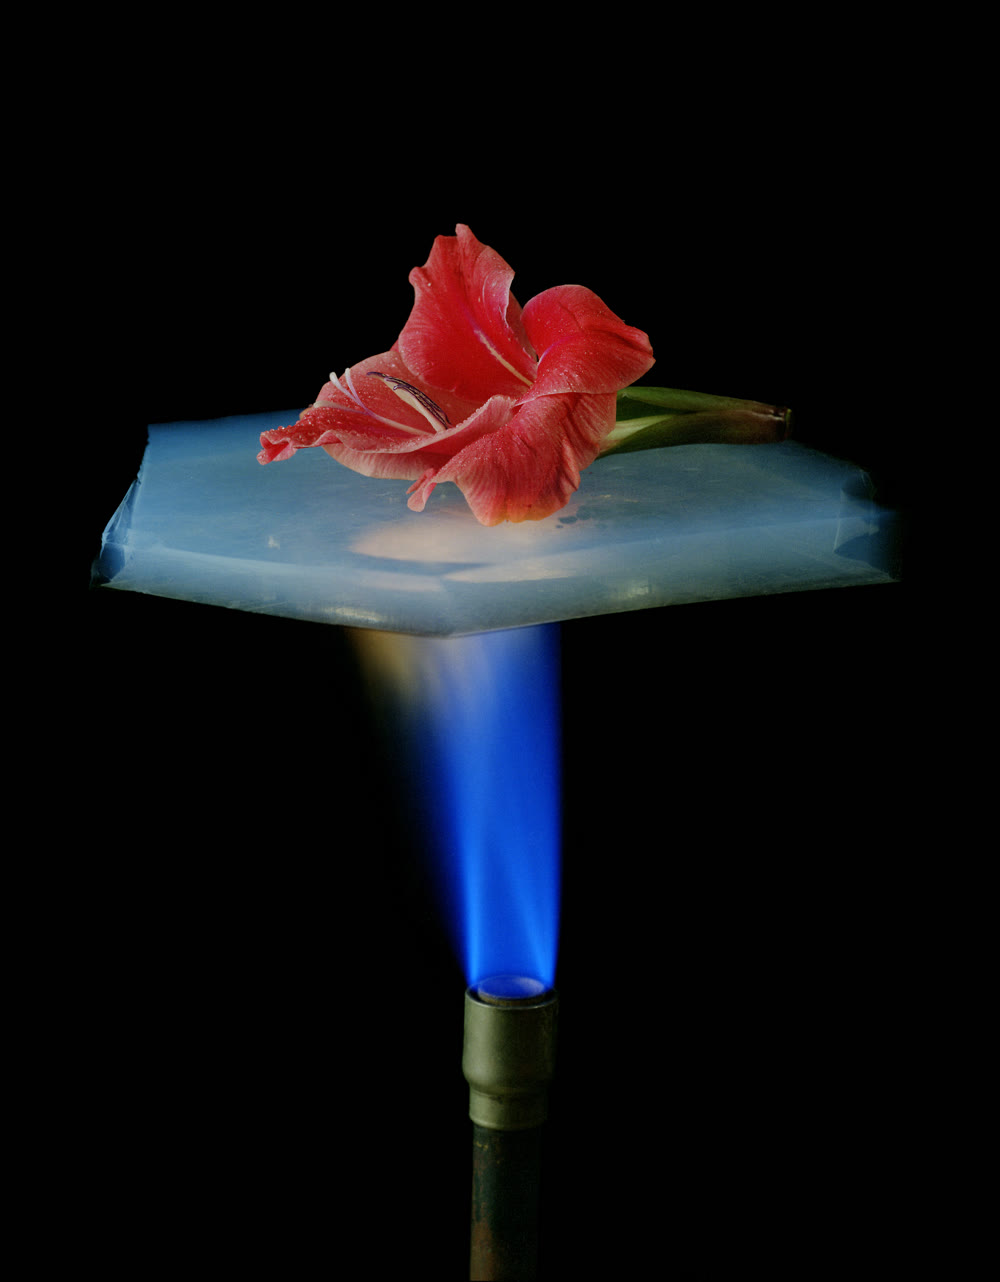
\includegraphics[width=0.38\linewidth]{images/book4/aerogel-flower.jpg}

{\small गैस ज्वाला के ऊपर सिलिका \omterm{def:b3:inorganic-materials:sol-gel}{एयरोजेल} की पट्टी पर एक फूल: \omterm{def:b3:inorganic-materials:sol-gel}{एयरोजेल}, एक
सुखाया हुआ \omterm{def:b3:colloids:colloid}{जेल} जो अधिकतर रिक्त स्थान है, ऊष्मा का बहुत कम चालन करता है। छायाचित्र:
NASA/JPL, सार्वजनिक अधिकार-क्षेत्र।}
\end{omfigure}

\section{संश्लेषण मार्ग}

\begin{definition}[सिरेमिक विधि]\label{def:b3:inorganic-materials:ceramic-method}
\emph{सिरेमिक विधि}\index{सिरेमिक विधि} ठोस अभिकारकों को एक साथ पीसकर
और उन्हें इतने उच्च तापों पर गर्म करके, प्रायः कई दिनों तक और
बार-बार पीसते हुए, कि आयन ठोसों से होकर विसरित हो सकें, एक ठोस यौगिक
बनाती है।
\end{definition}

दो ठोसों की अभिक्रिया उनके संपर्क पर होती है, और उत्पाद उनके बीच एक
परत बनाता है जिससे होकर फिर आयनों को जाना पड़ता है: सबसे धीमा चरण
विसरण है, और परत के मोटी होने के साथ यह धीमा होता जाता है।

\begin{proposition}[परवलयिक वृद्धि]\label{prop:b3:inorganic-materials:parabolic}
यदि किसी उत्पाद परत की वृद्धि उसके आर-पार विसरण द्वारा सीमित हो, तो उसकी
मोटाई $x^2 = kt$ के अनुसार बढ़ती है।
\end{proposition}

\begin{proof}
परत के दोनों फलकों पर नियत सांद्रताओं के साथ, उससे होकर फ़्लक्स
फ़िक के नियम, $J = D\Delta c/x$, का पालन करता है। परत फ़्लक्स के अनुपात में बढ़ती है:
$\dd x/\dd t = \lambda J = \lambda D\Delta c/x$, जहाँ $\lambda$ प्रति मोल परिवहित उत्पाद का आयतन है। तब
$x\,\dd x = \lambda D\Delta c\,\dd t$, और $x = 0$ से, $t = 0$ पर, समाकलन करने पर $x^2 = 2\lambda D\Delta c\,t = kt$ मिलता है।
\end{proof}

अतः कण आकार दुगुना करने से अभिक्रिया समय चार गुना हो जाता है: इसीलिए
महीन पिसाई, किसी पूर्वगामी में परमाणु पैमाने पर मिश्रण (एक मिश्रित ऑक्सैलेट या
सिट्रेट \omterm{def:b3:colloids:colloid}{जेल} जो विघटित होकर लक्ष्य बनता है), या एक विलयन मार्ग।

\begin{definition}[सॉल--जेल प्रक्रम]\label{def:b3:inorganic-materials:sol-gel}
\emph{सॉल--जेल प्रक्रम}\index{सॉल--जेल प्रक्रम} विलयन में आण्विक पूर्वगामियों, प्रायः
ऐल्कॉक्साइडों, के जल-अपघटन और संघनन द्वारा एक ऑक्साइड
बनाता है: विलयन छोटे ऑक्साइड गुच्छों का एक \omterm{def:b3:colloids:colloid}{सॉल} बनता है, फिर एक \omterm{def:b3:colloids:colloid}{जेल}, अर्थात्
द्रव से भरा एक सतत ठोस जाल। वाष्पन द्वारा सुखाने पर \omterm{def:b3:colloids:colloid}{जेल}
सिकुड़कर एक सघन \emph{ज़ीरोजेल}\index{ज़ीरोजेल} बनता है; द्रव के क्रांतिक
बिंदु से ऊपर सुखाने पर, जो द्रव--गैस अंतरापृष्ठ के बिना द्रव को हटा देता है, यह
\emph{एयरोजेल}\index{एयरोजेल} के रूप में अपना आयतन बनाए रखता है।
\end{definition}

\begin{omfigure}
\setchemfig{atom sep=2.0em}
\schemestart
\chemfig{RO-Si(-[2]OR)(-[6]OR)-OR}
\+ \chemfig{H_2O}
\arrow{->[जल-अपघटन]}[,1.4]
\chemfig{RO-Si(-[2]OR)(-[6]OR)-OH}
\+ ROH
\schemestop
\par\bigskip
\schemestart
\chemfig{{\equiv}Si-OH}
\+
\chemfig{HO-Si{\equiv}}
\arrow{->[संघनन]}[,1.6]
\chemfig{{\equiv}Si-O-Si{\equiv}}
\+ \chemfig{H_2O}
\schemestop
\par\medskip

{\small सिलिकॉन ऐल्कॉक्साइड का सॉल--जेल रसायन (R: एक ऐल्किल समूह,
टेट्राएथिल ऑर्थोसिलिकेट में एथिल): जल ऐल्कॉक्सी समूहों को हाइड्रॉक्सी समूहों से प्रतिस्थापित करता है, और
दो सिलानॉल संघनित होकर एक सिलॉक्सेन सेतु बनाते हैं। दोहराए जाने पर, संघनन
एक त्रिविमीय सिलिका जाल बनाते हैं।}
\end{omfigure}

पूर्ण अभिक्रिया के लिए दोनों अभिक्रियाएँ मिलकर देती हैं
$\ce{Si(OC2H5)4 + 2H2O -> SiO2 + 4C2H5OH}$। अम्ल उत्प्रेरण जल-अपघटन को तेज़ और
संघनन को धीमा बनाता है, जिससे पतले, शृंखला-जैसे बहुलक बनते हैं; क्षारक उत्प्रेरण
इसका उलटा, जिससे सघन कण बनते हैं। लेप (काँच पर प्रतिपरावर्तन परतें)
किसी भाग को \omterm{def:b3:colloids:colloid}{सॉल} में डुबोकर और बाहर खींचकर बनाए जाते हैं।

\begin{definition}[जलतापीय संश्लेषण]\label{def:b3:inorganic-materials:hydrothermal}
\emph{जलतापीय संश्लेषण}\index{जलतापीय संश्लेषण} किसी बंद पात्र में, जल के अपने
वाष्प दाब के अधीन, उसके सामान्य क्वथनांक से ऊपर के जल से एक ठोस को
क्रिस्टलित करता है; \emph{विलायकतापीय संश्लेषण}\index{विलायकतापीय संश्लेषण}
यही किसी अन्य विलायक में करता है।
\end{definition}

\begin{definition}[रासायनिक वाष्प निक्षेपण]\label{def:b3:inorganic-materials:cvd}
\emph{रासायनिक वाष्प निक्षेपण}\index{रासायनिक वाष्प निक्षेपण} (CVD) गैसीय पूर्वगामियों की
किसी गर्म पृष्ठ पर अभिक्रिया द्वारा उस पर एक ठोस फ़िल्म उगाता है, जैसे
सिलेन से सिलिकॉन, $\ce{SiH4 -> Si + 2H2}$, या मेथेन और हाइड्रोजन से हीरा।
\end{definition}

\begin{method}[संश्लेषण मार्ग का चयन]\label{met:b3:inorganic-materials:route}
\begin{enumerate}
  \item स्थूल चूर्ण के रूप में एक स्थायी, दुर्गलनीय ऑक्साइड: \omterm{def:b3:inorganic-materials:ceramic-method}{सिरेमिक विधि}, और यदि
        मिश्रण कठिन हो तो किसी पूर्वगामी के साथ।
  \item एक मितस्थायी प्रावस्था, एक महीन चूर्ण या निम्न ताप पर एक लेप:
        सॉल--जेल या अवक्षेपण।
  \item केवल गर्म जल में विलेय प्रावस्था के बड़े एकल क्रिस्टल (क्वार्ट्ज़) या
        किसी साँचे के चारों ओर बना ढाँचा (\omterm{def:b3:inorganic-materials:zeolite}{ज़िओलाइट}): जलतापीय।
  \item किसी आधार-पदार्थ पर एक पतली, शुद्ध फ़िल्म (\omterm{def:b3:solid-state:classes}{अर्धचालक} परतें): CVD।
\end{enumerate}
\end{method}

\begin{inthelab}[एक सॉल--जेल लेप और एक ऑटोक्लेव]
टेट्राएथिल ऑर्थोसिलिकेट को एथेनॉल, जल और अम्ल की एक बूँद के साथ तब तक विलोडित किया जाता है
जब तक विलयन स्वच्छ न हो जाए; एक साफ़ काँच की स्लाइड को उसमें डुबोकर
एक स्थिर धीमी गति से बाहर खींचा जाता है, सुखाया और गर्म किया जाता है, जिससे इतनी पतली सिलिका फ़िल्म बचती है कि
व्यतिकरण रंग दिखें। \omterm{def:b3:inorganic-materials:hydrothermal}{जलतापीय संश्लेषण} के लिए अभिकारकों को
पॉलिटेट्राफ़्लुओरोएथिलीन के एक अस्तर में रखा जाता है, जिसे लगभग दो-तिहाई से अधिक नहीं भरा जाता ताकि
फैलता द्रव पात्र को भर न दे, इस्पात के
ऑटोक्लेव में सीलबंद करके ओवन में गर्म किया जाता है; ऑटोक्लेव केवल ठंडा होने पर ही खोला जाता है।
\end{inthelab}

\begin{omfigure}
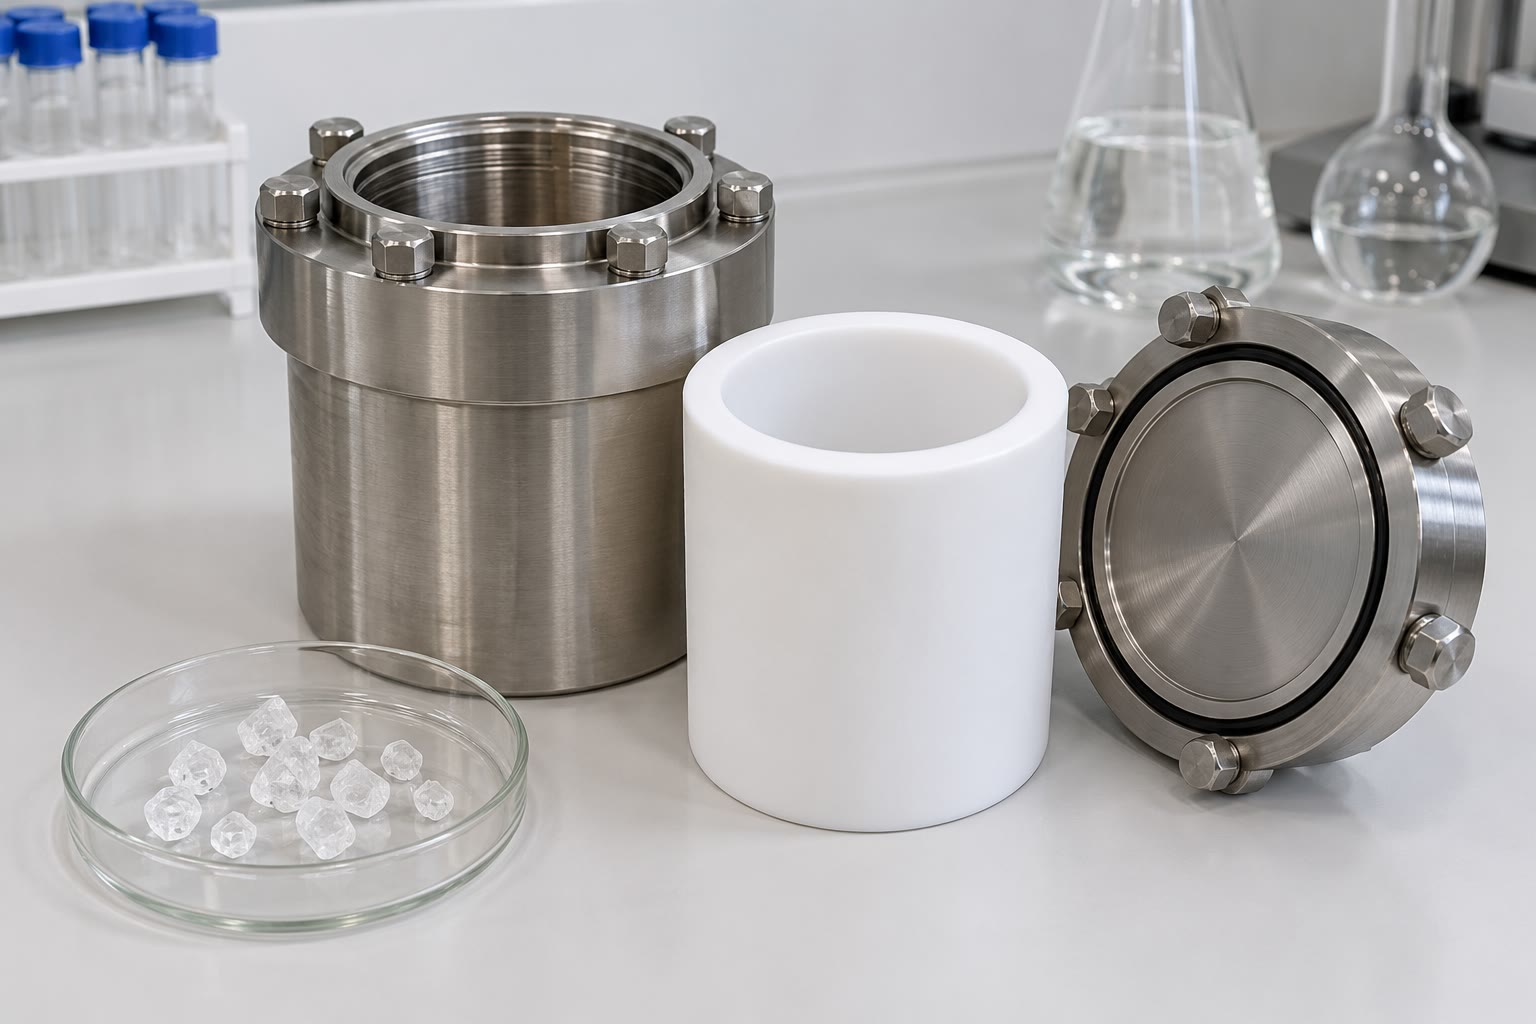
\includegraphics[width=0.5\linewidth]{images/book4/ai/b3-23-autoclave.jpg}

{\small \omterm{def:b3:inorganic-materials:hydrothermal}{जलतापीय संश्लेषण} के लिए एक प्रयोगशाला ऑटोक्लेव: बोल्ट से कसे ढक्कन वाला
इस्पात का खोल, अभिक्रिया मिश्रण धारण करने वाला सफ़ेद बहुलक अस्तर, और उसमें उगे
क्रिस्टल।}
\end{omfigure}

\section{सिरेमिक और काँच}

\begin{definition}[सिरेमिक]\label{def:b3:inorganic-materials:ceramic}
\emph{सिरेमिक}\index{सिरेमिक} किसी चूर्ण को गर्म करके बनाया गया एक अकार्बनिक, अधात्विक ठोस है:
ऑक्साइड, नाइट्राइड और कार्बाइड, या मृदा उत्पाद।
\end{definition}

\begin{definition}[पेरोव्स्काइट संरचना]\label{def:b3:inorganic-materials:perovskite}
किसी ऑक्साइड $\mathrm{ABO_3}$ की \emph{पेरोव्स्काइट संरचना}\index{पेरोव्स्काइट संरचना} में
छोटे B धनायन कोने साझा करने वाले $\mathrm{BO_6}$ अष्टफलकों के केंद्रों पर होते हैं और
बड़े A धनायन उनके बीच की द्वादश-उपसहसंयोजी गुहाओं में; आदर्श
घनीय कोष्ठिका में B केंद्र पर, O फलक केंद्रों पर, A कोनों पर होता है।
\emph{सह्यता गुणक}\index{सह्यता गुणक} मापता है कि आयन कितनी अच्छी तरह
समाते हैं:
\[
  t = \frac{r_A + r_O}{\sqrt2\,(r_B + r_O)}.
\]
\end{definition}

\begin{omfigure}
\tdplotsetmaincoords{60}{100}
\begin{tikzpicture}[tdplot_main_coords, scale=1.5, font=\small,
  aA/.style={om atom, ball color=green!45!black, minimum size=7.4mm},
  aB/.style={om atom, ball color=black!35, minimum size=4.4mm},
  aOs/.style={om atom, ball color=red!80, minimum size=4.8mm}]
  \pic[transform shape] {omcubeo={2}};
  % atoms back to front for view 60/100 (depth 0.853x + 0.150y + 0.5z)
  \node[aA] at (0,0,0) {};
  \node[aA] at (0,2,0) {};
  \node[aOs] (o1) at (0,1,1) {};
  \node[aA] at (0,0,2) {};
  \node[aOs] (o2) at (1,1,0) {};
  \node[aA] at (0,2,2) {};
  \node[aOs] (o3) at (1,0,1) {};
  \node[aB] (b) at (1,1,1) {};
  \node[aOs] (o4) at (1,2,1) {};
  \node[aA] at (2,0,0) {};
  \node[aOs] (o5) at (1,1,2) {};
  \node[aA] at (2,2,0) {};
  \node[aOs] (o6) at (2,1,1) {};
  \node[aA] at (2,0,2) {};
  \node[aA] at (2,2,2) {};
  \begin{scope}[on background layer]
    \draw[omMeth!70, line width=0.6pt] (o1.center) -- (o2.center) -- (o6.center) -- (o5.center) -- cycle
      (o3.center) -- (o2.center) -- (o4.center) -- (o5.center) -- cycle
      (o1.center) -- (o3.center) -- (o6.center) -- (o4.center) -- cycle;
    \draw[bond] (b.center) -- (o1.center) (b.center) -- (o2.center) (b.center) -- (o3.center)
      (b.center) -- (o4.center) (b.center) -- (o5.center) (b.center) -- (o6.center);
  \end{scope}
  \node[anchor=west] at (2,3.35,2) {A};
  \node[anchor=west] at (2,3.35,1) {O};
  \node[anchor=west] at (2,3.35,0) {B};
  \node[aA, minimum size=4mm] at (2,3.2,2) {};
  \node[aOs, minimum size=3.2mm] at (2,3.2,1) {};
  \node[aB, minimum size=3mm] at (2,3.2,0) {};
\end{tikzpicture}

{\small घनीय पेरोव्स्काइट कोष्ठिका $\mathrm{ABO_3}$: फलक केंद्रों पर स्थित छह ऑक्साइड आयनों के एक
अष्टफलक (हरे किनारे) के केंद्र पर एक B धनायन (धूसर), और A धनायन
कोनों पर। प्रत्येक कोने का A आयन आठ कोष्ठिकाओं द्वारा और प्रत्येक ऑक्सीजन
दो द्वारा साझा है: प्रति कोष्ठिका एक A, एक B और तीन O।}
\end{omfigure}

\begin{proposition}[आदर्श सह्यता गुणक]\label{prop:b3:inorganic-materials:tolerance}
आदर्श घनीय पेरोव्स्काइट में, जिसमें आयन B--O और A--O
दिशाओं के अनुदिश स्पर्श करते हैं, $t = 1$।
\end{proposition}

\begin{proof}
किनारे $a$ के साथ, केंद्र पर B और एक फलक केंद्र पर O, $a/2$ दूर हैं: $r_B + r_O = a/2$।
एक कोने पर A और संलग्न फलक के केंद्र पर O, आधे फलक विकर्ण की दूरी पर
हैं: $r_A + r_O = a\sqrt2/2$। भाग देने पर $(r_A + r_O)/(r_B + r_O) = \sqrt2$, अतः $t = 1$।
\end{proof}

जब $t$, 1 से थोड़ा कम होता है, तो A आयन अपनी गुहा के लिए बहुत छोटा होता है और
अष्टफलक उसके चारों ओर बंद होने के लिए झुक जाते हैं, जिससे सममिति घटती है; जब $t$, 1 से अधिक होता है,
तो B आयन अपने अष्टफलक के लिए बहुत छोटा होता है और केंद्र से हट सकता है।

\begin{definition}[लौहविद्युत]\label{def:b3:inorganic-materials:ferroelectric}
\emph{लौहविद्युत}\index{लौहविद्युत} ऐसा क्रिस्टल है जिसमें स्वतः
विद्युत ध्रुवण होता है, जिसे आरोपित विद्युत क्षेत्र उलट सकता है।
\end{definition}

% ledger: rion:Ba2+XII, rion:Ti4+VI, rion:O2-VI
बेरियम टाइटेनेट उत्कृष्ट उदाहरण है: $r(\ce{Ba^2+}) = \qty{161}{pm}$ (द्वादश-उपसहसंयोजी),
$r(\ce{Ti^4+}) = \qty{60.5}{pm}$ और $r(\ce{O^2-}) = \qty{140}{pm}$ के साथ, $t = 1.06$। एक संक्रमण ताप से नीचे
टाइटेनियम आयन केंद्र से हट जाते हैं, एक प्रक्षेत्र के भीतर सभी एक ही दिशा में,
और क्रिस्टल ध्रुवित हो जाता है; संक्रमण के निकट विशाल परावैद्युतांक
बेरियम टाइटेनेट को अधिकांश \omterm{def:b3:inorganic-materials:ceramic}{सिरेमिक} संधारित्रों का परावैद्युत बना देता है।

\begin{definition}[ऑक्साइड काँच]\label{def:b3:inorganic-materials:glass}
\emph{ऑक्साइड काँच}\index{ऑक्साइड काँच} एक अक्रिस्टलीय ऑक्साइड ठोस है, जो
किसी गलित को बिना क्रिस्टलन के ठंडा करके बनता है। इसके \emph{जाल
निर्माता}\index{जाल निर्माता} ($\ce{SiO2}$, $\ce{B2O3}$, $\ce{P2O5}$) कोने साझा करने वाले बहुफलकों का
एक सतत जाल बनाते हैं; इसके \emph{जाल रूपांतरक}\index{जाल रूपांतरक}
($\ce{Na2O}$, $\ce{CaO}$) उस जाल के सेतु तोड़ते हैं, प्रत्येक मिलाया गया ऑक्साइड आयन एक
सेतु ऑक्सीजन को दो असेतु ऑक्सीजनों में बदल देता है, और धनायन
छिद्रों में बैठते हैं।
\end{definition}

\begin{omfigure}
\begin{tikzpicture}
\begin{axis}[name=c, width=0.5\linewidth, axis equal image, hide axis, xmin=-1.2, xmax=12.6, ymin=-1.2, ymax=8.7]
\addplot[quiver={u=\thisrow{u}, v=\thisrow{v}}, -, black!60, line width=0.6pt] table {figdata/out/bachelor-3-glass-network-crystal-bonds.dat};
\addplot[only marks, mark=*, mark size=2.2pt, omDef] table {figdata/out/bachelor-3-glass-network-crystal-T.dat};
\addplot[only marks, mark=*, mark size=1.3pt, omThm, mark options={fill=white}] table {figdata/out/bachelor-3-glass-network-crystal-O.dat};
\end{axis}
\begin{axis}[at={(c.east)}, anchor=west, xshift=0.2cm, width=0.5\linewidth, axis equal image, hide axis, xmin=-1.2, xmax=12.6, ymin=-1.2, ymax=8.7]
\addplot[quiver={u=\thisrow{u}, v=\thisrow{v}}, -, black!60, line width=0.6pt] table {figdata/out/bachelor-3-glass-network-glass-bonds.dat};
\addplot[only marks, mark=*, mark size=2.2pt, omDef] table {figdata/out/bachelor-3-glass-network-glass-T.dat};
\addplot[only marks, mark=*, mark size=1.3pt, omThm, mark options={fill=white}] table {figdata/out/bachelor-3-glass-network-glass-O.dat};
\addplot[only marks, mark=*, mark size=1.5pt, omThm] table {figdata/out/bachelor-3-glass-network-glass-NBO.dat};
\addplot[only marks, mark=*, mark size=2.6pt, omProp] table {figdata/out/bachelor-3-glass-network-glass-Na.dat};
\end{axis}
\end{tikzpicture}

{\small समान संघटन के एक क्रिस्टल और एक काँच का द्विविमीय चित्र
(नीला: त्रि-उपसहसंयोजी निर्माता; खुले लाल वृत्त: सेतु
ऑक्सीजन)। बाएँ, क्रिस्टल एक ही वलय को दोहराता है। दाएँ, काँच: प्रत्येक निर्माता के
पास अब भी लगभग समान दूरियों पर तीन ऑक्सीजन हैं, परंतु वलयों में पाँच,
छह या सात सदस्य हैं और कुछ भी दोहराया नहीं जाता; दो स्थानों पर एक रूपांतरक ने एक
सेतु तोड़ दिया है, जिससे दो असेतु ऑक्सीजन (भरे लाल) और छिद्र में एक धनायन (नारंगी)
बचते हैं। स्प्रिंगों से विश्रांत मॉडल जाल।}
\end{omfigure}

विलियम ज़ाकारियासेन ने 1932 में तर्क दिया कि कोई ऑक्साइड आसानी से काँच बनाता है जब उसका
धनायन कम ऑक्सीजनों (तीन या चार) से घिरा हो, प्रत्येक ऑक्सीजन अधिक से अधिक
दो धनायनों को जोड़े, और बहुफलक कोने साझा करें, किनारे या फलक नहीं: तब एक
यादृच्छिक जाल की ऊर्जा क्रिस्टल से थोड़ी ही अधिक होती है। खिड़की का काँच
सोडियम और कैल्सियम ऑक्साइडों को रूपांतरक के रूप में लिए सिलिका है, जो गलन
ताप घटाते हैं। फ़ोनों के लिए कठोरीकृत आवरण काँच को गलित पोटैशियम
नाइट्रेट में भिगोया जाता है: बड़े $\ce{K+}$ आयन पृष्ठ में $\ce{Na+}$ आयनों का स्थान लेते हैं और, भीड़ के कारण,
उसे संपीडन में रखते हैं, ताकि दरारें न खुलें।

\section{सरंध्र ठोस: ज़िओलाइट और ढाँचे}

\begin{definition}[ज़िओलाइट]\label{def:b3:inorganic-materials:zeolite}
\emph{ज़िओलाइट}\index{ज़िओलाइट} एक क्रिस्टलीय ऐलुमिनोसिलिकेट है जिसका
कोने साझा करने वाले $\ce{SiO4}$ और $\ce{AlO4}$ चतुष्फलकों का ढाँचा आण्विक आकार के पिंजरे और
चैनल घेरता है, जिनके भीतर विनिमेय धनायन और जल होते हैं।
\emph{आण्विक चलनी}\index{आण्विक चलनी} वह सरंध्र ठोस है जो
अणुओं को उनके आकार के अनुसार प्रवेश देता है; \emph{आकृति वरणात्मकता}\index{आकृति वरणात्मकता}
उन रंध्रों के आकार और आकृति द्वारा किसी अभिक्रिया का नियंत्रण है जिनमें
वह होती है।
\end{definition}

प्रत्येक $\ce{AlO4}$ चतुष्फलक पर किसी $\ce{SiO4}$ की तुलना में एक ऋणावेश अधिक होता है
(सिलिकॉन(IV) के स्थान पर ऐलुमिनियम(III)); पिंजरों में स्थित धनायन, $\ce{Na+}$ या $\ce{Ca^2+}$,
इसे संतुलित करते हैं, और उनका विनिमय हो सकता है।

\begin{proposition}[लोवेनस्टाइन का नियम]\label{prop:b3:inorganic-materials:lowenstein}
किसी \omterm{def:b3:inorganic-materials:zeolite}{ज़िओलाइट} ढाँचे में दो $\ce{AlO4}$ चतुष्फलक कभी एक ऑक्सीजन साझा नहीं करते: Al--O--Al कड़ियाँ
अनुपस्थित होती हैं (सभी ज्ञात ऐलुमिनोसिलिकेट ढाँचों पर एक प्रेक्षण)। परिणामस्वरूप
किसी \omterm{def:b3:inorganic-materials:zeolite}{ज़िओलाइट} का अनुपात Si/Al कम से कम 1 होता है।
\end{proposition}

\begin{proof}[परिणाम की उपपत्ति]
प्रत्येक ऐलुमिनियम के चार ऑक्सीजन हैं, नियम के अनुसार प्रत्येक एक सिलिकॉन के साथ साझा:
$4N_{\mathrm{Al}}$ Al--O--Si कड़ियाँ। प्रत्येक सिलिकॉन के केवल चार ऑक्सीजन हैं, अतः वह अधिक से अधिक
चार ऐसी कड़ियों में भाग लेता है: $4N_{\mathrm{Al}} \le 4N_{\mathrm{Si}}$, अर्थात् $N_{\mathrm{Si}}/N_{\mathrm{Al}} \ge 1$। समता के लिए प्रत्येक
सिलिकॉन के चार ऐलुमिनियम पड़ोसी होने चाहिए: Si और Al एकांतर होते हैं।
\end{proof}

\begin{omfigure}
\tdplotsetmaincoords{55}{135}
\begin{tikzpicture}[tdplot_main_coords, scale=0.85, font=\small, baseline=(current bounding box.center),
  tSi/.style={circle, inner sep=0pt, minimum size=2.6mm, draw=black!70, fill=omDef!80},
  tAl/.style={circle, inner sep=0pt, minimum size=2.6mm, draw=black!70, fill=omProp!80}]
  % edges of a truncated octahedron (vertices: permutations of (0, +-1, +-2));
  % hidden edges (both faces facing away for this view) dashed
  \foreach \a/\b/\c/\d/\e/\f in {-2/-1/0/-2/0/-1, -2/-1/0/-2/0/1, -2/-1/0/-1/-2/0, -2/0/-1/-2/1/0, -2/0/-1/-1/0/-2, -1/-2/0/0/-2/-1, -1/-2/0/0/-2/1, -1/0/-2/0/-1/-2, -1/0/-2/0/1/-2, 0/-2/-1/0/-1/-2, 0/-2/-1/1/-2/0, 0/-1/-2/1/0/-2}
    \draw[black!40, dashed] (\a,\b,\c) -- (\d,\e,\f);
  \foreach \a/\b/\c/\d/\e/\f in {-2/0/1/-2/1/0, -2/0/1/-1/0/2, -2/1/0/-1/2/0, -1/0/2/0/-1/2, -1/0/2/0/1/2, -1/2/0/0/2/-1, -1/2/0/0/2/1, 0/-2/1/0/-1/2, 0/-2/1/1/-2/0, 0/-1/2/1/0/2, 0/1/-2/0/2/-1, 0/1/-2/1/0/-2, 0/1/2/0/2/1, 0/1/2/1/0/2, 0/2/-1/1/2/0, 0/2/1/1/2/0, 1/-2/0/2/-1/0, 1/0/-2/2/0/-1, 1/0/2/2/0/1, 1/2/0/2/1/0, 2/-1/0/2/0/-1, 2/-1/0/2/0/1, 2/0/-1/2/1/0, 2/0/1/2/1/0}
    \draw[black!75, line width=0.7pt] (\a,\b,\c) -- (\d,\e,\f);
  % T atoms back to front; hidden ones paler
  \foreach \x/\y/\z/\k/\v in {-2/-1/0/Si/0, -1/-2/0/Al/0, -2/0/-1/Al/0, 0/-2/-1/Si/0, -1/0/-2/Si/0, 0/-1/-2/Al/0, -2/0/1/Al/1, 0/-2/1/Si/1, -2/1/0/Si/1, 1/-2/0/Al/1, 0/1/-2/Al/1, 1/0/-2/Si/1, -1/0/2/Si/1, 0/-1/2/Al/1, -1/2/0/Al/1, 2/-1/0/Si/1, 0/2/-1/Si/1, 2/0/-1/Al/1, 0/1/2/Al/1, 1/0/2/Si/1, 0/2/1/Si/1, 2/0/1/Al/1, 1/2/0/Al/1, 2/1/0/Si/1}
    \node[t\k, opacity=0.35+0.65*\v] at (\x,\y,\z) {};
\end{tikzpicture}
\hspace{1.2cm}
\begin{tikzpicture}[font=\small, scale=0.8, baseline=(current bounding box.center)]
  \foreach \i in {0,1,2} \foreach \j in {0,1,2} {
    \fill[omDef!70] ($(2.2*\i,2.2*\j)+(-0.28,-0.28)$) rectangle +(0.56,0.56);
  }
  \foreach \i in {0,1} \foreach \j in {0,1,2} {
    \draw[black!70, line width=0.8pt] (2.2*\i+0.28,2.2*\j) -- (2.2*\i+0.75,2.2*\j);
    \draw[black!70, line width=0.8pt] (2.2*\i+1.45,2.2*\j) -- (2.2*\i+1.92,2.2*\j);
    \node[draw=black!70, regular polygon, regular polygon sides=6, minimum size=5.6mm, inner sep=0pt] at (2.2*\i+1.1,2.2*\j) {};
  }
  \foreach \i in {0,1,2} \foreach \j in {0,1} {
    \draw[black!70, line width=0.8pt] (2.2*\i,2.2*\j+0.28) -- (2.2*\i,2.2*\j+0.75);
    \draw[black!70, line width=0.8pt] (2.2*\i,2.2*\j+1.45) -- (2.2*\i,2.2*\j+1.92);
    \node[draw=black!70, regular polygon, regular polygon sides=6, minimum size=5.6mm, inner sep=0pt] at (2.2*\i,2.2*\j+1.1) {};
  }
  \node[font=\scriptsize, align=center] at (1.1,-0.85) {$\ce{Zn4O}$ नोड $+$ टेरेफ़्थैलेट संयोजक};
\end{tikzpicture}

{\small बाएँ: सोडालाइट पिंजरा, \omterm{def:b3:inorganic-materials:zeolite}{ज़िओलाइट} A की निर्माण इकाई, जिसके
प्रत्येक कोने पर एक चतुष्फलकीय परमाणु है (ऑक्सीजन, प्रत्येक किनारे के मध्य में,
नहीं दिखाए गए); सिलिकॉन (नीला) और ऐलुमिनियम (नारंगी) एकांतर हैं, जैसा लोवेनस्टाइन का नियम
Si/Al = 1 होने पर अपेक्षित करता है। दाएँ: एक \omterm{def:b3:inorganic-materials:mof}{धातु--कार्बनिक ढाँचे} की एक परत,
व्यवस्थात्मक: $\ce{Zn4O}$ गुच्छ (वर्ग), बेंज़ीन-1,4-डाइकार्बोक्सिलेट
संयोजकों (वलय) से जुड़कर बड़े रंध्रों वाला एक घनीय जाल बनाते हैं।}
\end{omfigure}

\begin{method}[ज़िओलाइट का सूत्र और विनिमय क्षमता]\label{met:b3:inorganic-materials:zeolite-formula}
\begin{enumerate}
  \item ढाँचे को $\mathrm{[(AlO_2)_x(SiO_2)_y]^{x-}}$ के रूप में लिखिए: Si/Al $= y/x$।
  \item ढाँचे का आवेश $-x$ धनायनों द्वारा संतुलित होता है: $x$ एकसंयोजी या $x/2$
        द्विसंयोजी।
  \item विनिमय क्षमता प्रति ग्राम विनिमेय आवेश की मात्रा है:
        $x/M$ मोल एकसंयोजी धनायन, $x/2M$ द्विसंयोजी, जहाँ $M$ तौले गए रूप में सूत्र का
        मोलर द्रव्यमान है (निर्जल या जलयोजित)।
\end{enumerate}
\end{method}

\begin{proposition}[विनिमय क्षमता]\label{prop:b3:inorganic-materials:exchange-capacity}
आवेश $z$ वाले धनायन के लिए किसी \omterm{def:b3:inorganic-materials:zeolite}{ज़िओलाइट} की क्षमता $x/(zM)$ मोल प्रति ग्राम है,
जहाँ $x$ मोलर द्रव्यमान $M$ वाले सूत्र में ऐलुमिनियम परमाणुओं की संख्या है।
\end{proposition}

\begin{proof}
प्रत्येक ऐलुमिनियम ढाँचे को एक ऋणावेश देता है; विद्युत
उदासीनता के लिए धनावेश की $x$ इकाइयाँ चाहिए, जो सभी विनिमेय हैं, अतः
$x/z$ धनायन, आवेश $z$ के, प्रति सूत्र इकाई, अर्थात् प्रति द्रव्यमान $M$।
\end{proof}

% ledger: iza:LTA.window, iza:MFI.channels
\omterm{def:b3:inorganic-materials:zeolite}{ज़िओलाइट} A में आठ चतुष्फलकों की खिड़कियाँ हैं, \qty{0.41}{nm} चौड़ी: जल और छोटे
आयन गुज़र जाते हैं, शाखित अणु नहीं। ZSM-5 में दस
चतुष्फलकों के चैनलों के दो समुच्चय हैं, लगभग 0.51 से \qty{0.56}{nm}: मेथेनॉल के रूपांतरण में या
टॉलूईन के ऐल्किलन में, पतला \textit{पैरा}-ज़ाइलीन अपने \textit{ऑर्थो} और \textit{मेटा} समावयवियों की तुलना में
कहीं तेज़ी से बाहर विसरित होता है, जो रुककर समावयवित होते रहते हैं। यही \omterm{def:b3:inorganic-materials:zeolite}{आकृति
वरणात्मकता} है।

\begin{definition}[धातु--कार्बनिक ढाँचे]\label{def:b3:inorganic-materials:mof}
\emph{धातु--कार्बनिक ढाँचा}\index{धातु--कार्बनिक ढाँचा} (MOF) धातु आयनों या गुच्छों से बना
एक क्रिस्टलीय ठोस है, जो बहुदंती कार्बनिक संयोजकों द्वारा एक सरंध्र जाल में जुड़े होते हैं।
\emph{द्वितीयक निर्माण
इकाई}\index{द्वितीयक निर्माण इकाई} अपने उपसहसंयोजी समूहों सहित धातु गुच्छ है,
जिसे जाल का एक नोड माना जाता है; \emph{जालिकीय
संश्लेषण}\index{जालिकीय संश्लेषण} दिए गए ज्यामिति के नोड और संयोजक चुनकर
किसी ढाँचे का ऐसा अभिकल्पन है कि वे एक चुने हुए जाल में संयोजित हों।
\end{definition}

% ledger: cod:MOF5.formula, cod:MOF5.a
MOF-5 में छह कार्बोक्सिलेट समूहों वाले $\ce{Zn4O}$ गुच्छ अष्टफलकीय नोड हैं,
और बेंज़ीन-1,4-डाइकार्बोक्सिलेट संयोजक उन्हें एक घनीय जाल के किनारों के अनुदिश
जोड़ते हैं, आठ नोडों की कोष्ठिका के लिए $a = \qty{25.82}{\angstrom}$। संयोजक को एक लंबे
संयोजक से बदलने पर जाल बना रहता है और रंध्र बड़े हो जाते हैं: यही जालिकीय विचार है। ऐसे
ढाँचों का पृष्ठीय क्षेत्रफल हज़ारों वर्ग मीटर प्रति ग्राम होता है और उनका
हाइड्रोजन और मेथेन के भंडारण तथा कार्बन डाइऑक्साइड के प्रग्रहण के लिए अध्ययन किया जाता है।

\begin{definition}[रंध्र आकार]\label{def:b3:inorganic-materials:pores}
% ledger: pore:micro, pore:macro
परिपाटी से, \emph{सूक्ष्मरंध्र}\index{सूक्ष्मरंध्र} \qty{2}{nm} से संकरे होते हैं,
\emph{मध्यरंध्र}\index{मध्यरंध्र} 2 और \qty{50}{nm} के बीच, और
\emph{स्थूलरंध्र}\index{स्थूलरंध्र} \qty{50}{nm} से चौड़े।
\end{definition}

\omterm{def:b3:inorganic-materials:zeolite}{ज़िओलाइट} और अधिकांश MOF सूक्ष्मरंध्री हैं; सिलिका \omterm{def:b3:colloids:colloid}{जेल} और \omterm{def:b3:inorganic-materials:sol-gel}{एयरोजेल} मध्यरंध्री।

\section{नैनोकण}

\begin{definition}[नैनोपदार्थ]\label{def:b3:inorganic-materials:nano}
\emph{नैनोपदार्थ}\index{नैनोपदार्थ} की कम से कम एक विमा लगभग
1 और \qty{100}{nm} के बीच होती है; \emph{नैनोकण}\index{नैनोकण} की
तीनों।
\end{definition}

\begin{proposition}[जादुई गुच्छ]\label{prop:b3:inorganic-materials:magic}
एक केंद्रीय परमाणु और $n$ पूर्ण कोशों से बने घनअष्टफलकीय गुच्छ में
\[
  N(n) = \frac{10n^3 + 15n^2 + 11n + 3}{3}
\]
परमाणु होते हैं, जिनमें से $10n^2 + 2$ पृष्ठ पर हैं: 13, 55, 147, 309, \dots
\end{proposition}

\begin{proof}
घनअष्टफलक के $k$-वें कोश में 12 शीर्ष, 24 किनारे जिनमें से प्रत्येक के भीतर $k - 1$ परमाणु,
8 त्रिभुजाकार फलक जिनमें से प्रत्येक में $(k - 1)(k - 2)/2$ आंतरिक परमाणु, और 6
वर्गाकार फलक जिनमें $(k - 1)^2$ हैं: कुल $12 + 24(k - 1) + 4(k - 1)(k - 2) + 6(k - 1)^2 = 10k^2 + 2$। तब
$N(n) = 1 + \sum_{k=1}^{n}(10k^2 + 2) = 1 + \frac{10n(n + 1)(2n + 1)}{6} + 2n$, जिसका विस्तार सूत्र देता है;
बाहरी कोश, $10n^2 + 2$ परमाणु, पृष्ठ है।
\end{proof}

\begin{omfigure}
\begin{tikzpicture}
\begin{axis}[name=a, width=0.47\linewidth, height=5.4cm, xmin=0, xmax=18, ymin=0, ymax=1,
  axis lines=left, xlabel={व्यास / \unit{nm}}, ylabel={पृष्ठ पर परमाणुओं का अंश},
  tick label style={font=\scriptsize}, label style={font=\small}]
\addplot[omDef, thick, mark=*, mark size=1pt] table[x=diam_nm, y=fsurf] {figdata/out/bachelor-3-nanoparticle-size.dat};
\end{axis}
\begin{axis}[at={(a.east)}, anchor=west, xshift=1.5cm, width=0.47\linewidth, height=5.4cm,
  xmin=0.8, xmax=6, ymin=0, ymax=3, axis lines=left,
  xlabel={त्रिज्या $R$ / \unit{nm}}, ylabel={परिरोधन ऊर्जा / \unit{eV}},
  tick label style={font=\scriptsize}, label style={font=\small}]
\addplot[omThm, thick] table[x=R_nm, y=dE_eV] {figdata/out/bachelor-3-nanoparticle-size-b.dat};
\end{axis}
\end{tikzpicture}

{\small बाएँ: घनअष्टफलकीय स्वर्ण गुच्छों के पृष्ठ पर परमाणुओं का अंश,
उनके व्यास के विरुद्ध: लगभग \qty{3}{nm} से छोटे गुच्छों के लिए आधे से अधिक,
\qty{8}{nm} पर अब भी पाँचवाँ भाग। दाएँ: गोलाकार \omterm{def:b3:inorganic-materials:quantum-dot}{क्वांटम बिंदु} में एक
इलेक्ट्रॉन--कोटर युग्म की परिरोधन ऊर्जा (मॉडल \omterm{def:b3:quantum-model-systems:oscillator}{समानीत द्रव्यमान} $0.10\,m_e$),
जो \omterm{def:b3:solid-state:band}{बैंड अंतराल} में जुड़ती है और $1/R^2$ के अनुसार गिरती है।}
\end{omfigure}

अपने परमाणुओं के एक बड़े अंश के पृष्ठ पर होने से, जहाँ उनके कम
पड़ोसी होते हैं, कोई \omterm{def:b3:inorganic-materials:nano}{नैनोकण} स्थूल धातु की तुलना में निम्नतर ताप पर पिघलता है,
अधिक क्रियाशील होता है, और कहीं बेहतर उत्प्रेरक हो सकता है: स्थूल स्वर्ण अक्रिय है, जबकि
कुछ नैनोमीटर चौड़े स्वर्ण कण कक्ष ताप पर कार्बन मोनोऑक्साइड का ऑक्सीकरण करते हैं।

\begin{definition}[क्वांटम बिंदु]\label{def:b3:inorganic-materials:quantum-dot}
\emph{क्वांटम बिंदु}\index{क्वांटम बिंदु} इतना छोटा \omterm{def:b3:solid-state:classes}{अर्धचालक} नैनोक्रिस्टल है
कि उसके इलेक्ट्रॉनों और \omterm{def:b3:solid-state:carriers}{कोटरों} का परिरोधन उसके \omterm{def:b3:solid-state:band}{बैंड अंतराल} को
स्थूल ठोस के अंतराल से ऊपर उठा देता है।
\end{definition}

\begin{theorem}[गोले में परिरोधन]\label{thm:b3:inorganic-materials:quantum-dot}
द्रव्यमान $m$ का एक कण, जो अनंत दीवारों द्वारा त्रिज्या $R$ के गोले में परिरुद्ध हो,
मूल-अवस्था ऊर्जा $E = \hbar^2\pi^2/(2mR^2) = h^2/(8mR^2)$ रखता है, तरंग फलन $\psi \propto \sin(\pi r/R)/r$ के साथ।
\end{theorem}

\begin{proof}
गोलीय सममित अवस्था $\psi(r) = u(r)/r$ के लिए लाप्लासी देता है
$\nabla^2\psi = u''/r$, अतः भीतर \omterm{thm:b3:quantum-model-systems:schrodinger}{श्रोडिंगर समीकरण} $-\frac{\hbar^2}{2m}u'' = Eu$ बन जाता है, जो एक रेखा पर
कण का समीकरण है। केंद्र पर परिमित $\psi$ वाले हल के लिए $u(0) = 0$: $u = \sin(kr)$, $E = \hbar^2k^2/2m$ के साथ।
दीवार $u(R) = 0$ माँगती है, अतः मूल अवस्था के लिए $kR = \pi$, और $E = \hbar^2\pi^2/(2mR^2)$।
\end{proof}

किसी बिंदु में इलेक्ट्रॉन और \omterm{def:b3:solid-state:carriers}{कोटर} दोनों परिरुद्ध होते हैं; निम्नतम
उत्तेजन की ऊर्जा प्रथम सन्निकटन में $E_g + h^2/(8\mu R^2)$ है, जहाँ $\mu$ उनका \omterm{def:b3:quantum-model-systems:oscillator}{समानीत
द्रव्यमान} है (उनका कूलॉम आकर्षण इसे थोड़ा घटाता है)। त्रिज्या आधी करने से
परिरोधन ऊर्जा चार गुना हो जाती है: कुछ नैनोमीटर के कैडमियम सेलेनाइड बिंदु
केवल आकार के अनुसार लाल, हरे या नीले चमकते हैं, और डिस्प्ले में
उत्सर्जकों के रूप में प्रयुक्त होते हैं।

\begin{definition}[पृष्ठ प्लाज़्मॉन अनुनाद]\label{def:b3:inorganic-materials:plasmon}
\emph{पृष्ठ प्लाज़्मॉन अनुनाद}\index{पृष्ठ प्लाज़्मॉन अनुनाद} प्रकाश द्वारा चालित,
किसी धातु \omterm{def:b3:inorganic-materials:nano}{नैनोकण} के चालन इलेक्ट्रॉनों का सामूहिक दोलन है; यह एक प्रबल अवशोषण बैंड देता है जिसकी तरंगदैर्ध्य
धातु, कण के आकार और आकृति तथा उसके परिवेश पर निर्भर करती है।
\end{definition}

कुछ दसियों नैनोमीटर के स्वर्ण \omterm{def:b3:inorganic-materials:nano}{नैनोकण} हरा प्रकाश अवशोषित करते हैं और काँच या \omterm{def:b3:colloids:colloid}{कोलॉइड} में
माणिक-लाल दिखते हैं; उनके समुच्चयित होने पर बैंड लंबी
तरंगदैर्ध्यों की ओर खिसकता है और रंग नीला हो जाता है: अनेक त्वरित परीक्षणों का आधार, जिनमें
प्रतिपिंड-लेपित स्वर्ण \omterm{def:b3:colloids:colloid}{कोलॉइड} एक रंगीन रेखा में एकत्र होता है।

\section{कार्बन नैनोपदार्थ}

\begin{definition}[कार्बन नैनोपदार्थ]\label{def:b3:inorganic-materials:carbon}
\emph{फ़ुलरीन}\index{फ़ुलरीन} कार्बन परमाणुओं का एक बंद पिंजरा अणु है,
जिसमें प्रत्येक परमाणु तीन अन्य से आबंधित है, पंच- और षट्सदस्यीय वलयों के साथ, जैसे
विंशफलकीय $\ce{C60}$। \emph{कार्बन नैनोनली}\index{कार्बन नैनोनली} ग्रेफ़ाइट की एक
चादर है जिसे लगभग एक नैनोमीटर चौड़े निर्बाध बेलन में लपेटा गया हो।
\emph{ग्रैफ़ीन}\index{ग्रैफ़ीन} ग्रेफ़ाइट की एक अकेली परत है, एक परमाणु मोटी।
\end{definition}

\begin{proposition}[बारह पंचभुज]\label{prop:b3:inorganic-materials:euler}
प्रत्येक \omterm{def:b3:inorganic-materials:carbon}{फ़ुलरीन} में ठीक बारह पंचभुज होते हैं, उसके षट्भुजों की संख्या
चाहे जो हो।
\end{proposition}

\begin{proof}
एक बंद पिंजरा एक बहुफलक है: ऑयलर का सूत्र $V - E + F = 2$ लागू होता है। प्रत्येक परमाणु के
तीन आबंध हैं और प्रत्येक आबंध के दो परमाणु: $2E = 3V$। $p$ पंचभुजों और $h$ षट्भुजों के साथ,
फलकों से किनारे गिनने पर $2E = 5p + 6h$, और $F = p + h$। तब $V = 2E/3$ और ऑयलर का
सूत्र $-E/3 + p + h = 2$ बनता है, अर्थात् $-(5p + 6h)/6 + p + h = 2$, अतः $p/6 = 2$: $p = 12$।
\end{proof}

\begin{omfigure}
\begin{tikzpicture}[scale=0.62, font=\small]
  \def\hexd{0.6}
  \begin{scope}
    \clip (-0.4,-0.5) rectangle (9.6,5.2);
    \foreach \i in {-3,...,10} \foreach \j in {-1,...,6} {
      \pgfmathsetmacro\cx{1.7320508*\hexd*(\i + 0.5*\j)}
      \pgfmathsetmacro\cy{1.5*\hexd*\j}
      \draw[black!45] ({\cx+\hexd*cos(30)},{\cy+\hexd*sin(30)})
        \foreach \k in {90,150,...,390} { -- ({\cx+\hexd*cos(\k)},{\cy+\hexd*sin(\k)}) };
    }
  \end{scope}
  \draw[->, thick, omDef] (0,0) -- ({1.7320508*\hexd},0) node[below right, font=\scriptsize, fill=white, inner sep=1pt] {$\mathbf a_1$};
  \draw[->, thick, omDef] (0,0) -- ({1.7320508*\hexd*0.5},{1.5*\hexd}) node[left, font=\scriptsize, fill=white, inner sep=1pt] {$\mathbf a_2$};
  \draw[->, very thick, omThm] (0,0) -- ({1.7320508*\hexd*(4+0.5*2)},{1.5*\hexd*2}) node[above right, font=\scriptsize, fill=white, inner sep=1pt] {$\mathbf C_h = 4\mathbf a_1 + 2\mathbf a_2$};
  \draw[dashed, omMeth, thick] (0,0) -- ({1.7320508*\hexd*9},0) node[right, font=\scriptsize] {ज़िगज़ैग $(n, 0)$};
  \draw[dashed, omProp, thick] (0,0) -- ({1.7320508*\hexd*5*1.5},{1.5*\hexd*5}) node[below right, font=\scriptsize, fill=white, inner sep=1pt] {आरामकुर्सी $(n, n)$};
\end{tikzpicture}

{\small एक \omterm{def:b3:inorganic-materials:carbon}{ग्रैफ़ीन} चादर और किसी नैनोनली का किरैल सदिश: चादर को इस प्रकार लपेटने पर
कि $\mathbf C_h = n\mathbf a_1 + m\mathbf a_2$ का सिरा उसके मूल से मिले, $(n, m)$ नली मिलती है, यहाँ $(4, 2)$।
$\mathbf a_1$ के अनुदिश $(n, 0)$ नली का किनारा ज़िगज़ैग है; $\mathbf a_1 + \mathbf a_2$ के अनुदिश, 30° पर, $(n, n)$
नली का किनारा आरामकुर्सी है।}
\end{omfigure}

\begin{proposition}[धात्विक और अर्धचालक नैनोनलियाँ]\label{prop:b3:inorganic-materials:nanotube}
एकल-भित्ति \omterm{def:b3:inorganic-materials:carbon}{कार्बन नैनोनली} $(n, m)$ धात्विक होती है जब $n - m$, 3 का गुणज हो, और
अन्यथा \omterm{def:b3:solid-state:classes}{अर्धचालक}। \admitted
\end{proposition}

इस प्रकार सभी संभव नलियों में से एक-तिहाई धात्विक हैं, जिनमें हर आरामकुर्सी
नली सम्मिलित है; अन्य का अंतराल उनके व्यास के बढ़ने के साथ गिरता है। स्वयं \omterm{def:b3:inorganic-materials:carbon}{ग्रैफ़ीन} में
कोई अंतराल नहीं होता: उसके संयोजकता और \omterm{def:b3:solid-state:band}{चालन बैंड} एकल बिंदुओं पर स्पर्श करते हैं, और उसके
इलेक्ट्रॉन ऐसे गति करते हैं मानो उनका कोई द्रव्यमान न हो।

\begin{safety}{\ghs[0.62cm]{GHS02}\ghs[0.62cm]{GHS07}\ghs[0.62cm]{GHS08}}
% ledger: ghs4:TEOS
टेट्राएथिल ऑर्थोसिलिकेट: ज्वलनशील द्रव और वाष्प, साँस द्वारा लेने पर हानिकारक,
आँखों और श्वसन मार्गों के लिए उत्तेजक; धूम-हुड में सँभाला जाता है। नैनोचूर्ण:
सबसे महीन कण फेफड़ों में गहराई तक पहुँचते हैं, और अनेक अभी वर्गीकृत नहीं हैं;
उन्हें एक आवरण में या निलंबन के रूप में तौला और सँभाला जाता है, खुली वायु में
ढीली धूल के रूप में कभी नहीं।
\end{safety}

\begin{omfigure}
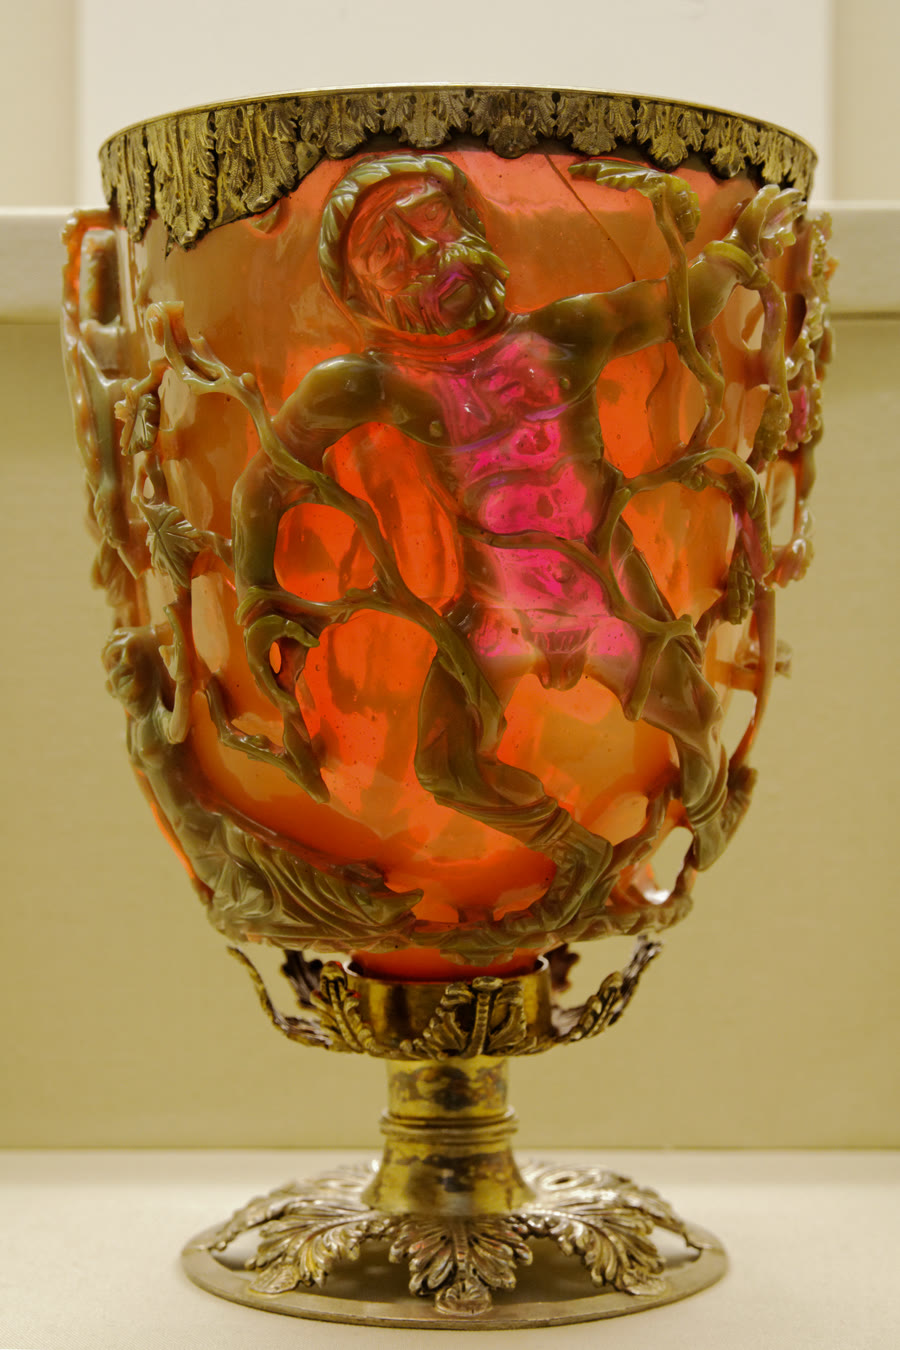
\includegraphics[width=0.32\linewidth]{images/book4/lycurgus-cup.jpg}

{\small भीतर से प्रकाशित लाइकर्गस प्याला, चौथी शताब्दी का एक रोमन काँच:
यह परावर्तित प्रकाश में हरा और पारगत प्रकाश में लाल दिखता है, जो काँच में
स्वर्ण--रजत \omterm{def:b3:inorganic-materials:nano}{नैनोकणों} का प्रभाव है। छायाचित्र: मारी-लान न्गुयेन, CC BY
2.5।}
\end{omfigure}

\begin{history}[शब्द से पहले के नैनोकण, और कार्बन की एक फ़ुटबॉल]
काँच बनाने वाले यह जाने बिना ही कि क्यों, बहुत पहले से स्वर्ण द्वारा काँच को लाल रंगते थे;
लाइकर्गस प्याला इस प्रभाव को सबसे आकर्षक रूप में दिखाता है। माइकल फ़ैराडे ने 1850 के दशक में स्वर्ण
\omterm{def:b3:colloids:colloid}{कोलॉइड} बनाए और देखा कि उनका रंग इतने छोटे कणों से आता है जो
दिखाई नहीं देते। 1985 में हैरल्ड क्रोटो, रॉबर्ट कर्ल और रिचर्ड स्मॉली ने, लेज़र से
ग्रेफ़ाइट को वाष्पित करते हुए, पाया कि साठ कार्बन परमाणुओं के गुच्छ
असाधारण रूप से स्थायी थे और बारह पंचभुजों तथा
बीस षट्भुजों का बंद पिंजरा प्रस्तावित किया; उन्हें रसायन का 1996 का नोबेल पुरस्कार मिला।
\end{history}

\section{अभ्यास}

\begin{exercise}[$\star$]\label{exo:b3:inorganic-materials:1}
दो ठोसों के बीच एक उत्पाद परत \qty{10}{h} के बाद \qty{2.0}{\micro\metre} मोटी है। यदि वृद्धि परवलयिक हो, तो
\qty{6.0}{\micro\metre} मोटी होने में कितना समय लगेगा?
\end{exercise}

\begin{exercise}[$\star$]\label{exo:b3:inorganic-materials:2}
टेट्राएथिल ऑर्थोसिलिकेट का सिलिसिक अम्ल में जल-अपघटन, सिलिसिक अम्ल के दो अणुओं का
संघनन, और सिलिका देने वाली समग्र अभिक्रिया लिखिए।
\end{exercise}

\begin{exercise}[$\star$]\label{exo:b3:inorganic-materials:3}
$\ce{SiO2}$, $\ce{B2O3}$, $\ce{Na2O}$ और $\ce{CaO}$ को \omterm{def:b3:inorganic-materials:glass}{जाल निर्माताओं} या रूपांतरकों के रूप में वर्गीकृत कीजिए, और बताइए कि
$\ce{Na2O}$ सिलिका के जाल के साथ क्या करता है।
\end{exercise}

\begin{exercise}[$\star$]\label{exo:b3:inorganic-materials:4}
$\ce{C70}$ में कितने पंचभुज और षट्भुज हैं? कितने आबंध?
\end{exercise}

\begin{exercise}[$\star\star$]\label{exo:b3:inorganic-materials:5}
% ledger: rion:Sr2+XII, rion:Ca2+XII, rion:Ba2+XII, rion:Ti4+VI, rion:O2-VI
$\ce{SrTiO3}$, $\ce{BaTiO3}$ और $\ce{CaTiO3}$ के \omterm{def:b3:inorganic-materials:perovskite}{सह्यता गुणक} परिकलित कीजिए, द्वादश-उपसहसंयोजी त्रिज्याओं
$\ce{Sr^2+}$ (\qty{144}{pm}), $\ce{Ba^2+}$ (\qty{161}{pm}) और $\ce{Ca^2+}$ (\qty{134}{pm}), $r(\ce{Ti^4+}) = \qty{60.5}{pm}$ और $r(\ce{O^2-}) = \qty{140}{pm}$ के साथ। वे
क्या पूर्वानुमान करते हैं?
\end{exercise}

\begin{exercise}[$\star\star$]\label{exo:b3:inorganic-materials:6}
एक \omterm{def:b3:inorganic-materials:zeolite}{ज़िओलाइट} X का निर्जल सूत्र $\mathrm{Na_{86}[(AlO_2)_{86}(SiO_2)_{106}]}$ है (अभ्यास के आँकड़े)।
Si/Al और $\ce{Ca^2+}$ के लिए उसकी विनिमय क्षमता मिलीमोल प्रति ग्राम में बताइए।
\end{exercise}

\begin{exercise}[$\star\star$]\label{exo:b3:inorganic-materials:7}
% ledger: lat:Au
स्वर्ण फलक-केंद्रित घनीय है, $a = \qty{407.8}{pm}$। लगभग \qty{5}{nm} चौड़े एक
घनअष्टफलकीय स्वर्ण कण के कोशों की संख्या, उसके परमाणुओं की संख्या और
उसके पृष्ठ पर अंश का आकलन कीजिए।
\end{exercise}

\begin{exercise}[$\star\star$]\label{exo:b3:inorganic-materials:8}
एक \omterm{def:b3:solid-state:classes}{अर्धचालक} का स्थूल अंतराल \qty{1.74}{eV} है, और उसके इलेक्ट्रॉन और \omterm{def:b3:solid-state:carriers}{कोटर} का \omterm{def:b3:quantum-model-systems:oscillator}{समानीत
द्रव्यमान} $0.10\,m_e$ (अभ्यास के आँकड़े)। कूलॉम आकर्षण की उपेक्षा करते हुए, 2.0 और \qty{3.0}{nm} त्रिज्या वाले
बिंदुओं द्वारा उत्सर्जित प्रकाश के रंग का आकलन कीजिए।
\end{exercise}

\begin{exercise}[$\star\star$]\label{exo:b3:inorganic-materials:9}
नैनोनलियाँ $(10, 10)$, $(10, 0)$, $(9, 0)$ और $(12, 8)$ धात्विक हैं या \omterm{def:b3:solid-state:classes}{अर्धचालक}? कौन-सी
आरामकुर्सी हैं, कौन-सी ज़िगज़ैग?
\end{exercise}

\begin{exercise}[$\star\star\star$]\label{exo:b3:inorganic-materials:10}
% ledger: cod:MOF5.formula, cod:MOF5.a, cod:MOF5.Z
MOF-5, $\mathrm{Zn_4O(C_8H_4O_4)_3}$, घनीय है, $a = \qty{25.82}{\angstrom}$ और प्रति कोष्ठिका आठ सूत्र इकाइयों के साथ।
इसका घनत्व परिकलित कीजिए। यदि एक ग्राम का पृष्ठीय क्षेत्रफल $\qty{3000}{m^2}$ हो (अभ्यास के
आँकड़े), तो यह $\qty{105}{m} \times \qty{68}{m}$ के कितने फ़ुटबॉल मैदानों के बराबर है?
\end{exercise}

\begin{exercise}[$\star\star\star$]\label{exo:b3:inorganic-materials:11}
\cref{prop:b3:inorganic-materials:magic} की कोश-गणना का उपयोग करके दिखाइए कि
किसी घनअष्टफलकीय गुच्छ का पृष्ठ अंश $3/n$ की ओर प्रवृत्त होता है, बड़े $n$ के लिए, और
$n = 8$ के लिए यथार्थ अंश से इसकी तुलना कीजिए।
\end{exercise}

\begin{exercise}[$\star\star\star$]\label{exo:b3:inorganic-materials:12}
प्रति परमाणु तीन आबंधों वाले एक बंद कार्बन पिंजरे में $p$ पंचभुज, $h$ षट्भुज
और $s$ सप्तभुज हैं। दिखाइए कि $p - s = 12$।
\end{exercise}

\section{समस्या: ज़िओलाइट A से जल का मृदुकरण}

\begin{problem}[{सप्ताहांत समस्या --- ज़िओलाइट A से जल का मृदुकरण:
सूत्र और लोवेनस्टाइन का नियम, सैद्धांतिक विनिमय क्षमता, एक धुलाई के लिए
आवश्यक ज़िओलाइट, और वह खिड़की जो कैल्सियम को भीतर आने देती है और अपमार्जकों को
बाहर रखती है}]
\label{pb:b3:inorganic-materials:1}
% ledger: iza:LTA.formula, iza:LTA.window, aw:Na, aw:Al, aw:Si, aw:O, aw:H, aw:Ca, aw:C, rion:Ca2+VI
\omterm{def:b3:inorganic-materials:zeolite}{ज़िओलाइट} A, जो अपमार्जकों में फ़ॉस्फ़ेटों के स्थान पर प्रयुक्त होता है, का सूत्र
$\mathrm{Na_{12}[(AlO_2)_{12}(SiO_2)_{12}]\cdot 27H_2O}$ है और खिड़कियाँ \qty{0.41}{nm} चौड़ी हैं। नल के एक जल में
$\ce{Ca^2+}$ का \qty{2.0}{mmol/L} है, और एक धुलाई में उसका \qty{15}{L} प्रयुक्त होता है; एक धुलाई के समय में \omterm{def:b3:inorganic-materials:zeolite}{ज़िओलाइट}
अपनी क्षमता के 60\,\% तक पहुँचता है (समस्या के आँकड़े)।

\medskip\noindent\textbf{भाग I --- सूत्र।}
\begin{enumerate}
  \item निर्जल सूत्र का मोलर द्रव्यमान परिकलित कीजिए।
  \item जलयोजित सूत्र का मोलर द्रव्यमान परिकलित कीजिए।
  \item Si/Al बताइए।
  \item लोवेनस्टाइन का नियम बताइए और यह भी कि यहाँ Si और Al की व्यवस्था के लिए
        इसका क्या अर्थ है।
  \item प्रति सूत्र ढाँचे का आवेश क्या है?
  \item जलयोजित \omterm{def:b3:inorganic-materials:zeolite}{ज़िओलाइट} में जल का द्रव्यमान अंश परिकलित कीजिए।
\end{enumerate}

\medskip\noindent\textbf{भाग II --- विनिमय क्षमता।}
\begin{enumerate}[resume]
  \item सोडियम \omterm{def:b3:inorganic-materials:zeolite}{ज़िओलाइट} और कैल्सियम
        आयनों के बीच विनिमय साम्य लिखिए।
  \item एक सूत्र कितने $\ce{Ca^2+}$ ग्रहण कर सकता है?
  \item निर्जल \omterm{def:b3:inorganic-materials:zeolite}{ज़िओलाइट} की सैद्धांतिक क्षमता mmol $\ce{Ca^2+}$
        प्रति ग्राम में परिकलित कीजिए।
  \item जलयोजित \omterm{def:b3:inorganic-materials:zeolite}{ज़िओलाइट} के लिए इसे परिकलित कीजिए।
  \item निर्जल क्षमता को मिलीग्राम $\ce{CaCO3}$ प्रति ग्राम में व्यक्त कीजिए, जो जल की कठोरता की सामान्य
        इकाई है।
\end{enumerate}

\medskip\noindent\textbf{भाग III --- एक धुलाई।}
\begin{enumerate}[resume]
  \item एक धुलाई के जल में $\ce{Ca^2+}$ की मात्रा परिकलित कीजिए।
  \item सैद्धांतिक क्षमता पर आवश्यक जलयोजित \omterm{def:b3:inorganic-materials:zeolite}{ज़िओलाइट} का द्रव्यमान परिकलित कीजिए।
  \item क्षमता के 60\,\% पर इसे परिकलित कीजिए।
  \item जल में मुक्त हुए सोडियम का द्रव्यमान परिकलित कीजिए।
  \item अपमार्जक निर्माताओं ने फ़ॉस्फ़ेटों को क्यों बदला?
  \item \omterm{def:b3:inorganic-materials:zeolite}{ज़िओलाइट} A, $\ce{Mg^2+}$ को $\ce{Ca^2+}$ की तुलना में अधिक धीरे क्यों ग्रहण करता है?
\end{enumerate}

\medskip\noindent\textbf{भाग IV --- खिड़की।}
\begin{enumerate}[resume]
  \item खिड़की की तुलना किसी $\ce{Ca^2+}$ आयन के व्यास (षट्-उपसहसंयोजी त्रिज्या
        \qty{100}{pm}) से कीजिए।
  \item गुज़रने के लिए किसी जलयोजित $\ce{Ca^2+}$ आयन को क्या करना होगा?
  \item डोडेसिल सल्फ़ेट जैसा कोई \omterm{def:b3:colloids:surfactant}{पृष्ठसक्रियक} ऋणायन बाहर क्यों रह जाता है?
  \item शोषक कारक के रूप में \omterm{def:b3:inorganic-materials:zeolite}{ज़िओलाइट} A क्या करता है, और इसे
        \omterm{def:b3:inorganic-materials:zeolite}{आण्विक चलनी} क्यों कहा जाता है?
  \item $\ce{Na+}$ को $\ce{K+}$ से बदलने पर प्रवेश पाने वाले अणुओं का आकार कैसे बदलेगा?
  \item ZSM-5 में \textit{पैरा}-ज़ाइलीन रंध्रों को \textit{ऑर्थो}-ज़ाइलीन से तेज़ी से क्यों छोड़ता है?
  \item परिणाम बताइए: $\ce{Ca^2+}$ के लिए निर्जल \omterm{def:b3:inorganic-materials:zeolite}{ज़िओलाइट} A की सैद्धांतिक विनिमय
        क्षमता।
\end{enumerate}
\end{problem}
